\documentclass[11pt,a4paper]{article}
\usepackage[utf8]{inputenc}
\usepackage[spanish]{babel}
\usepackage{amsmath}
\usepackage{amsfonts}
\usepackage{amssymb}
\usepackage{graphicx}
\usepackage{pdfpages}
\usepackage[left=2cm,right=2cm,top=2cm,bottom=2cm]{geometry}
\author{Valdez Bernal Maria Fernanda\\Valdez Esquivel Melani Betsabee\\
González Pardo Adrian}

\title{Reporte de practica 2}
\newcommand\tab[1][1cm]{\hspace*{#1}}
\begin{document}
\maketitle
\section{Introducción}
El uso de semáforos se puede aplicar de varias maneras para
generar lo que es un proceso de datos mas grandes o en paralelo, por bloques o simplemente para ver la eficiencia de un algoritmo para cierto problema a resolver.\\
Para el desarrollo de esta practica se utilizaron semáforos e hilos para hacer las producciones de datos y así mismo consumir dichos datos, aun no hay un ejemplo en aplicación muy claro pero si lo pasamos a lo que es enviar y recibir datos de un usuario en red, podemos decir que hay cinco servidores y cinco clientes, de los cuales quieren extraer $x$ o $y$ dato, nosotros gestionamos dichos servidores y consumidores para que haya un orden en como se va dando la interacción de datos usuario y así sea de manera mas eficaz y rápida para ambas partes, claro sin sobrepasar las imitaciones del equipo o del equipo del usuario.\\
EL uso de semáforos nuevamente nos ayuda a tener una gestión de nuestro proceso de manera local y global, pensar primero en cuantos vamos a necesitar para controlar cada proceso es parte de la solución, en este caso usamos (2 semáforos)
\section{Desarrollo}

Para iniciar el problema planteado es que 5 productores necesitan producir datos de los conjuntos $A=\{a,b,c,d,e\}$ y $B=\{1,2,3,4,5\}$ en y tienen 2 secciones de 4 espacios para hacerlo, con la condición de primero deben producir un dato del conjunto A en la primera sección y luego les sera permitido de producir un dato del conjunto B en l segunda sección y así el numero de veces que se haya pedido (en este caso es para una prueba inicial de 10,000 datos). Los consumidores, al llegar a los datos lo irán poniendo en archivos de texto, donde habrá 10 archivos, cinco para letras, cinco para números.\\
En este caso resolvimos el problema pensando en el uso de 11 semáforos, primero que nada un semáforo por cada valor en la sección critica, para ir controlando que se produce y que se va bloqueando conforme se va usando, es decir el semáforo 1 sera para controlar la sección del productor y el semáforo 2 del consumidor, pero sin dejar de lado que cada bloque de as secciones tendrá su propio semáforo, también la parte de los consumidores para mandar a archivos txt tendrá su propio semáforo para ir enviando los datos que consuma en el proceso y los escriba en dichos archivos.\\
Para el control de los datos que se van consumiendo y mandado a los archivos, utilizamos apoyo de lo que es un Script desarrollado en bash, el cual permite visualizar en pantalla el número de datos entrantes de cada archivo, así como el asegurarse que los datos que debe insertar el programa por cada productor sean los datos correctos.

\subsection{Diagrama de flujo}
\begin{center}
    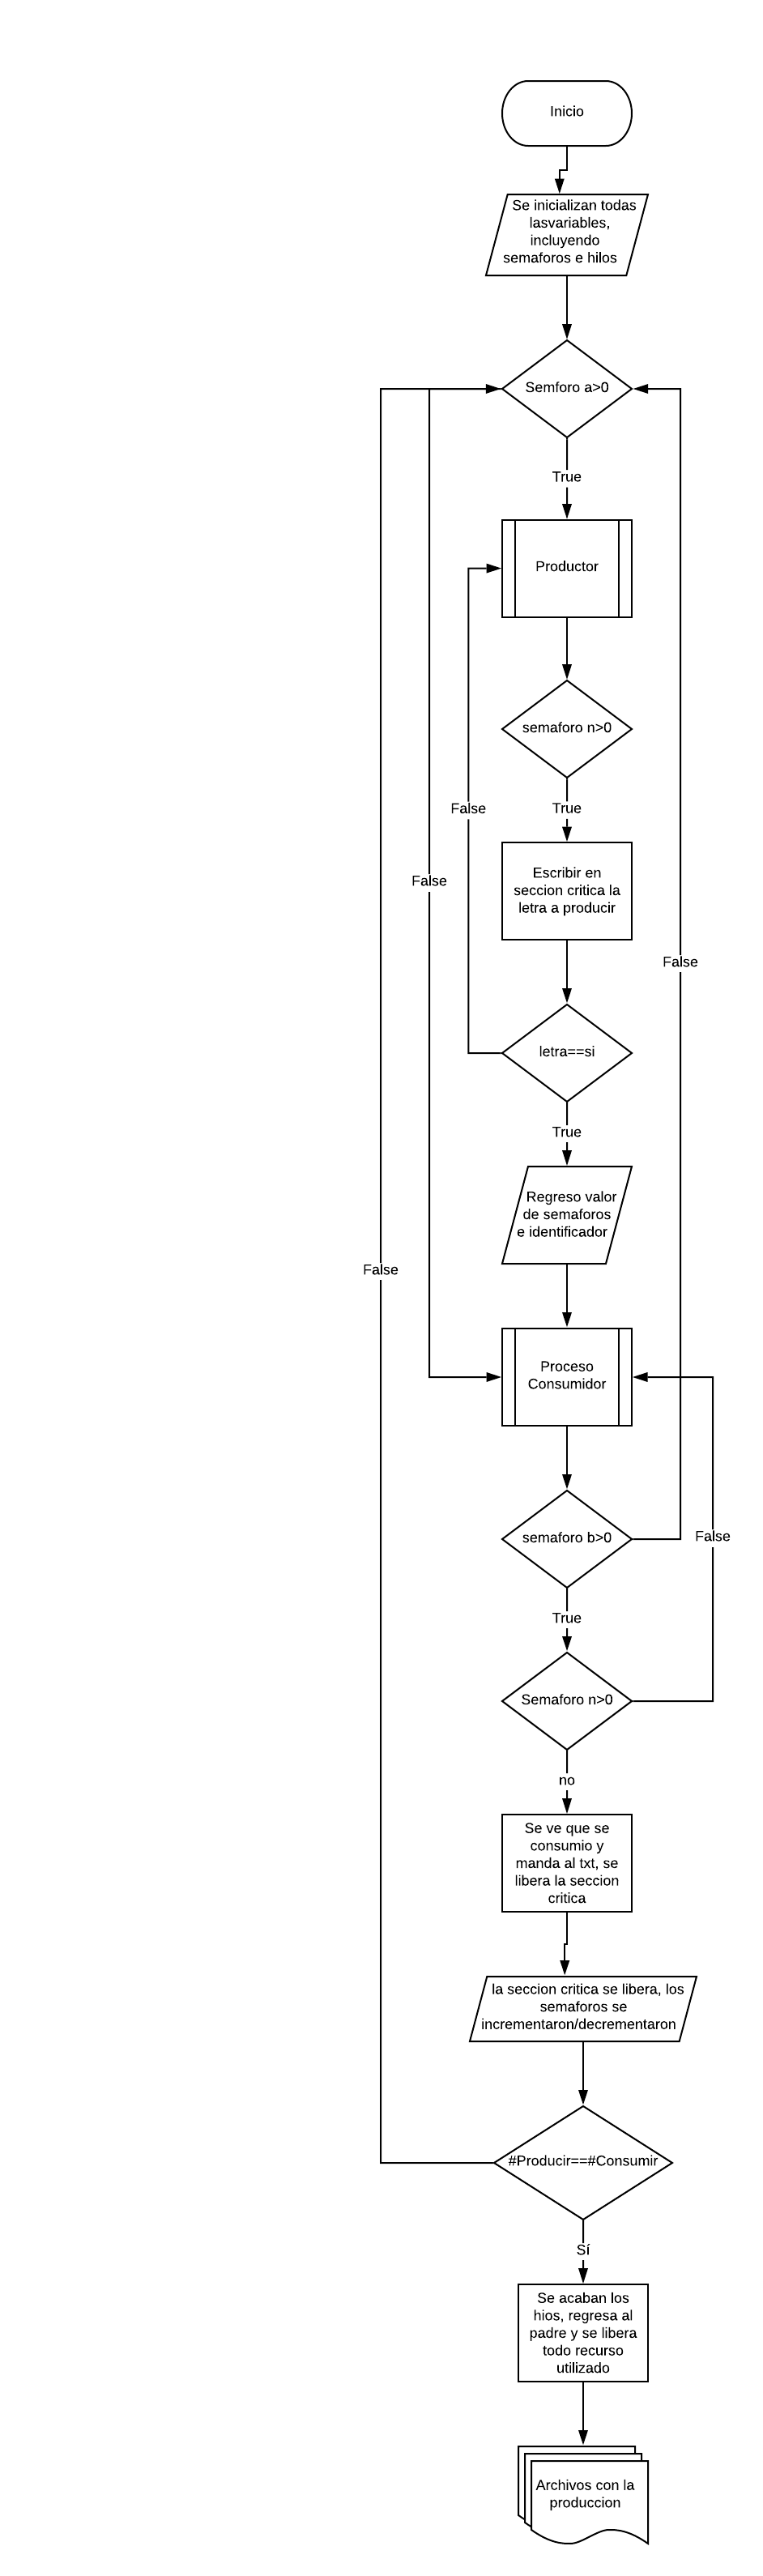
\includegraphics[scale=0.5]{imgs/estaxd.png}
    \\
    \textit{Figura del diagrama de flujo de datos para la solución del problema.}
\end{center}

El diagrama de datos nos ayuda a entender un poco el desarrollo del problema, ya que de primera instancia podemos observar que se declaran e inicializan las variables\\
Se van a crear 11 semáforos de los cuales, 8 son para las secciones criticas, así aplicaremos 4 a cada sección y a su vez cada sección podrá monitorizar x,y,z,v de cada sección para hacer independiente a cada producción y a cada consumidor.\\
Una vez que se hizo la creación de los semáforos y de los hilos (un hilo para el productor y un hilo para el consumidor) se procede a ir  dichas funciones y realizar lo que nos muestra el diagrama.\\
Primero se verifica el estado del semáforo controlador de dicha sección, si este esta abierto se procede a verificar los semáforos de cada sección de esta parte para ver en cual de todas se puede producir siempre y cuando dicho productor ya haya producido una letra atentes para ingresar a la sección de los números. Dicho proceso se produce las 10,000 veces y se pasa a l función de consumidor.\\
En la función del consumidor se verifica si su semáforo esta abierto, de ser así se verifica el semáforo que nos ayuda a controlar los 10 archivos de txt y una vez que se consumió se procede a liberar dicha sección de donde tomo el dato.\\
Una vez que productor y consumidor han terminado se procede a liberar todos los recursos que se han ocupado, es decir, se destruyen los semáforos y se liberan los hilos, asi mismo como la memoria que se llegase a ocupar en el proceso.

\subsection{Valdez Esquivel Melani Betsabee}
%Así van los comentarios y puedes escribir así directamente
El uso de semáforos, es bastante útil para todo tipo de aplicaciones, desde una aplicación donde se deban resguardar secciones de código (secciones criticas) hasta las API's para hacer uso de las redes, con este ejemplo podemos notar que puede haber mas de un subproceso que sea una sección critica, como es el caso de los archivos de texto, en primera instancia nos marcan 2 secciones para los productores y consumidores, pero para poder manejar los archivos de texto también tuvimos que ver esa parte como una sección critica y también usar semáforos para controlar lo que se va escribiendo en ellos.

\subsection{González Pardo Adrian}
Gracias al uso de semáforos que nos permite hacer uso de sincronización de procesos y/o de  hilos, nos funciona mucho para hacer aplicaciones que nos permitan resolver diversas problemáticas que en tiempo de ejecución lineal, pueden tardar alrededor de tiempos exageradamente grandes en los que el hacer uso de modularidad y de separar vía cómputo paralelo o concurrente pueden reducir el tiempo de ejecución y de completar la tarea haciendo uso de todo el poder que el hardware de computo de multinucleo o multihilo nos proporciona, acorde a sus nuevas tecnologías e implementaciones.






\end{document}
